\documentclass{beamer}
\usepackage[utf8]{inputenc}

\usetheme{Madrid}
\usecolortheme{default}
\usepackage{amsmath,amssymb,amsfonts,amsthm}
\usepackage{txfonts}
\usepackage{tkz-euclide}
\usepackage{listings}
\usepackage{adjustbox}
\usepackage{array}
\usepackage{tabularx}
\usepackage{gvv}
\usepackage{lmodern}
\usepackage{circuitikz}
\usepackage{tikz}
\usepackage[utf8]{inputenc}

\usetheme{Madrid}
\usecolortheme{default}
\usepackage{amsmath,amssymb,amsfonts,amsthm}
\usepackage{txfonts}
\usepackage{tkz-euclide}
\usepackage{listings}
\usepackage{adjustbox}
\usepackage{array}
\usepackage{tabularx}
\usepackage{gvv}
\usepackage{lmodern}
\usepackage{circuitikz}
\usepackage{tikz}
\usepackage{graphicx}

\setbeamertemplate{page number in head/foot}[totalframenumber]

\usepackage{tcolorbox}
\tcbuselibrary{minted,breakable,xparse,skins}



\definecolor{bg}{gray}{0.95}
\DeclareTCBListing{mintedbox}{O{}m!O{}}{%
  breakable=true,
  listing engine=minted,
  listing only,
  minted language=#2,
  minted style=default,
  minted options={%
    linenos,
    gobble=0,
    breaklines=true,
    breakafter=,,
    fontsize=\small,
    numbersep=8pt,
    #1},
  boxsep=0pt,
  left skip=0pt,
  right skip=0pt,
  left=25pt,
  right=0pt,
  top=3pt,
  bottom=3pt,
  arc=5pt,
  leftrule=0pt,
  rightrule=0pt,
  bottomrule=2pt,

  colback=bg,
  colframe=orange!70,
  enhanced,
  overlay={%
    \begin{tcbclipinterior}
    \fill[orange!20!white] (frame.south west) rectangle ([xshift=20pt]frame.north west);
    \end{tcbclipinterior}},
  #3,
}
\lstset{
    language=C,
    basicstyle=\ttfamily\small,
    keywordstyle=\color{blue},
    stringstyle=\color{orange},
    commentstyle=\color{green!60!black},
    numbers=left,
    numberstyle=\tiny\color{gray},
    breaklines=true,
    showstringspaces=false,
}
%------------------------------------------------------------
%This block of code defines the information to appear in the
%Title page
\title %optional
{5.2.17}
\date{September  2025}
%\subtitle{A short story}

\author % (optional)
{Bhoomika L - EE25BTECH11014}

\begin{document}


\frame{\titlepage}
\begin{frame}{Question}
Solve the given system of linear equations:
\begin{center}
    $x-3y-7=0$\\$3x-3y-15=0$
\end{center}
\end{frame}

\begin{frame}{Solution}
The given equations of line can be expressed as:\\
\begin{align}
    \vec{n^T}\vec{x}=c\\
    \myvec{1&-3}\myvec{x\\y}=7\\
 \myvec{3 &-3}\myvec{x\\y}=15
 \end{align}

 The matrix we get by the above equations is as follows:
\begin{align}
     \myvec{1&-3\\3&-3}\myvec{x\\y}=\myvec{7\\15}
\end{align}
\end{frame}

\begin{frame}{Solution}
 The following is the augmented matrix which can be solved using Gaussian elimination.
 \begin{align}
       \myvec{\begin{array}{cc|c}
1 & -3 & 7 \\ 
3 & -3 & 15\end{array}} \xrightarrow{\;R_2\longrightarrow R_2-3R_1\;}       \myvec{\begin{array}{cc|c}
1 & -3 & 7 \\ 
0 & 6 & -6\end{array}}\\
\myvec{\begin{array}{cc|c}
1 & -3 & 7 \\ 
0 & 6 & -6\end{array}} \xrightarrow{\;R_2\longrightarrow \frac{R_2}{6}\;}
\myvec{\begin{array}{cc|c}
1 & -3 & 7 \\ 
0 & 1 & -1\end{array}}\\
\myvec{\begin{array}{cc|c}
1 & -3 & 7 \\ 
0 & 1 & -1\end{array}} \xrightarrow{\;R_1\longrightarrow R_1+3R_2\;} \myvec{\begin{array}{cc|c}
1 & 0 & 4 \\ 
0 & 1 & -1\end{array}} 
\end{align}
\end{frame}


\begin{frame}{Solution}
    From the matrix,\\
\begin{align}
    \myvec{1&0\\0&1}\myvec{x\\y}=\myvec{4\\-1}\\
    \therefore \myvec{x\\y}=\myvec{4\\-1}
\end{align}
\end{frame}

\begin{frame}{Plot}
    \centering
    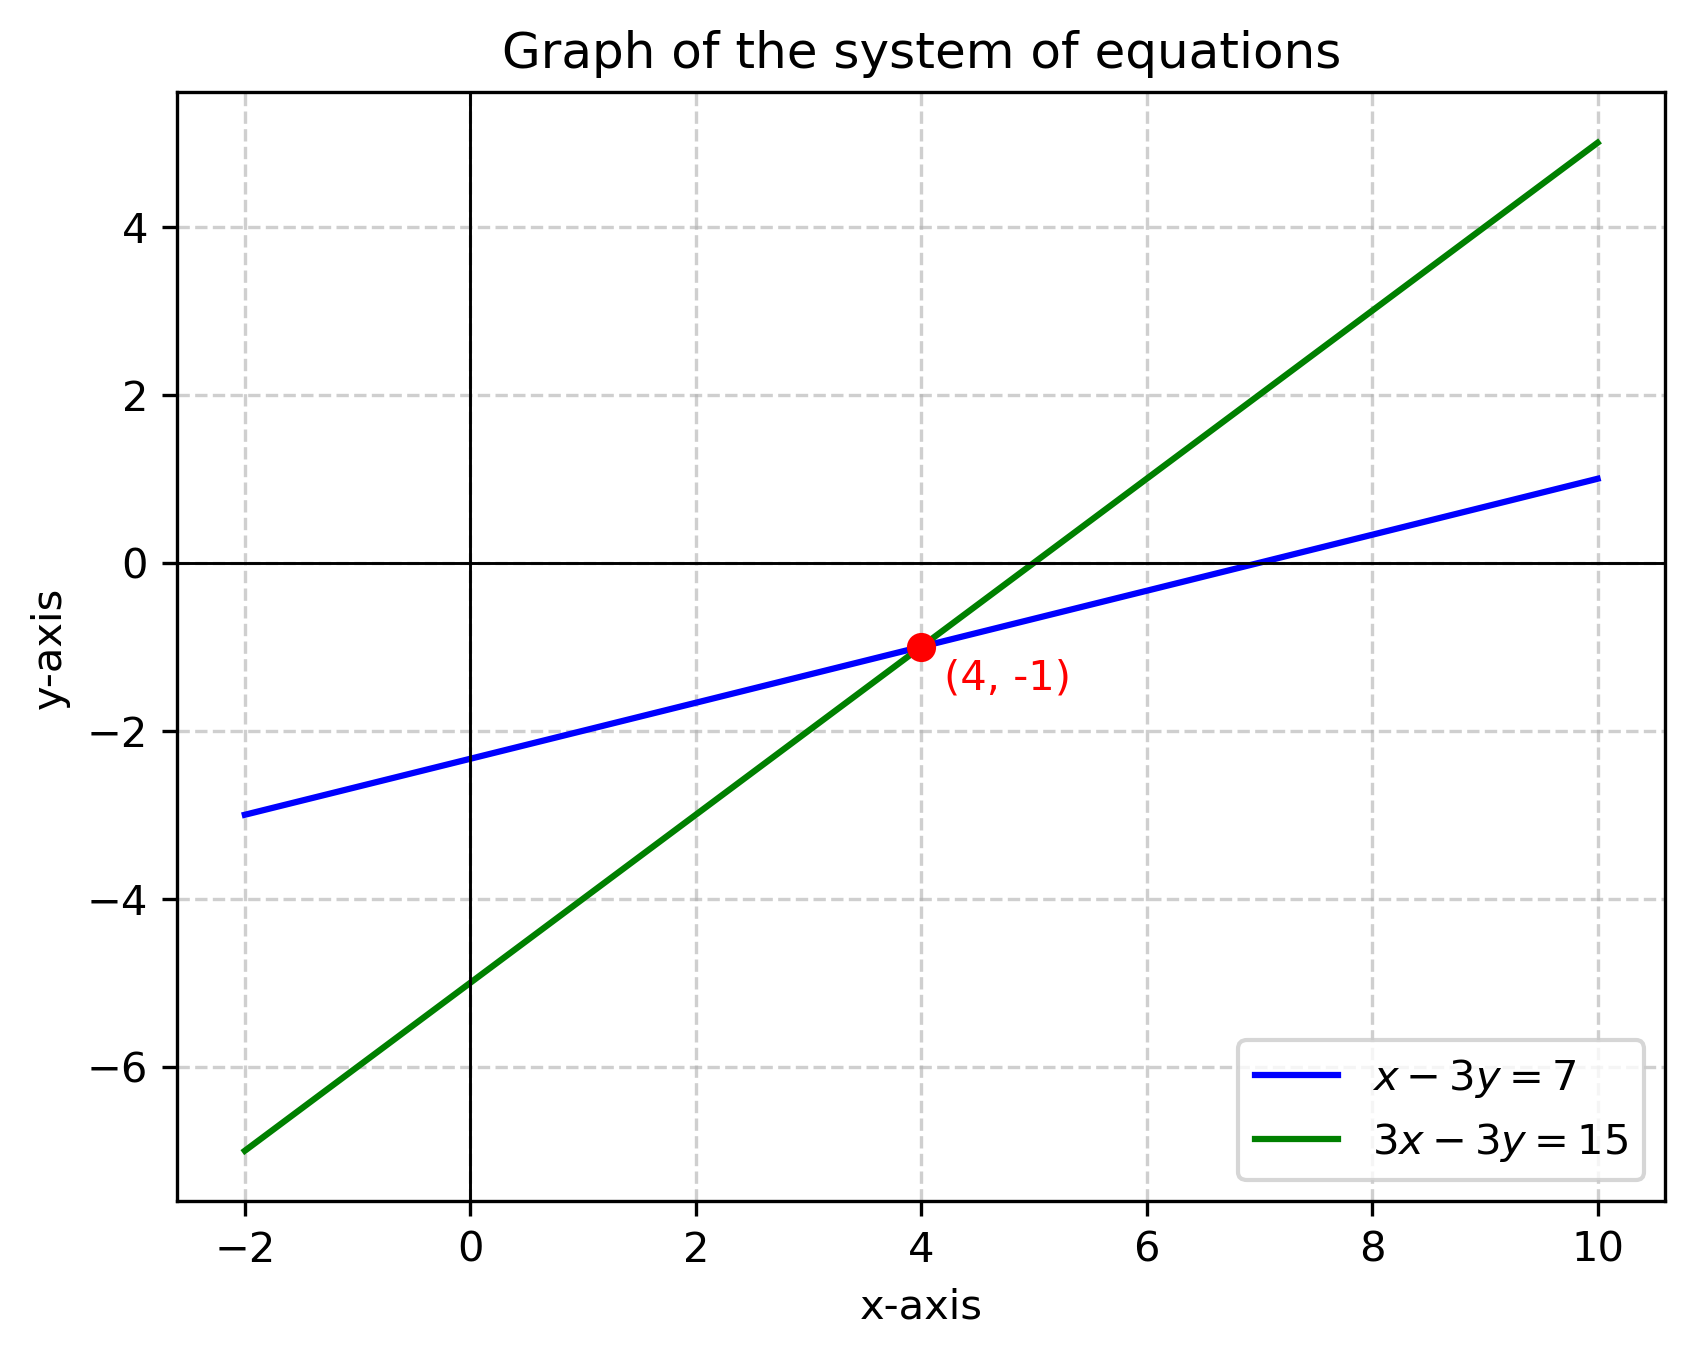
\includegraphics[width=\columnwidth, height=0.8\textheight, keepaspectratio]{../Figs/LE.png}     
\end{frame}

 \begin{frame}[fragile]
\frametitle{C Code }
\begin{lstlisting}
    #include <stdio.h>

// Solve system of equations:
// x - 3y = 7
// 3x - 3y = 15
//
// Returns solution in sol[0] = x, sol[1] = y
void solve_system(double sol[2]) {
    double a11 = 1, a12 = -3, b1 = 7;
    double a21 = 3, a22 = -3, b2 = 15;

    double det = a11 * a22 - a12 * a21;

    sol[0] = (b1 * a22 - a12 * b2) / det;  // x
    sol[1] = (a11 * b2 - b1 * a21) / det;  // y
}

\end{lstlisting}
\end{frame}

 \begin{frame}[fragile]
\frametitle{Python Code }
\begin{lstlisting}
import ctypes
import numpy as np
import matplotlib.pyplot as plt

# Load the shared library
lib = ctypes.CDLL("./code.so")

# Define argument and return types
lib.solve_system.argtypes = [np.ctypeslib.ndpointer(dtype=np.double, ndim=1, flags="C_CONTIGUOUS")]
lib.solve_system.restype = None

 # Prepare array to hold solution [x, y]
sol = np.zeros(2, dtype=np.double)

\end{lstlisting}
\end{frame}

 \begin{frame}[fragile]
\frametitle{Python Code }
\begin{lstlisting}
# Call the C function
lib.solve_system(sol)

# Print result
print("Solution of system:")
print("x =", sol[0])
print("y =", sol[1])

# Define the two equations in terms of y
# x - 3y = 7  =>  y = (x - 7)/3
# 3x - 3y = 15  =>  y = x - 5
def line1(x):
    return (x - 7) / 3

def line2(x):
    return x - 5
\end{lstlisting}
\end{frame}

 \begin{frame}[fragile]
\frametitle{Python Code }
\begin{lstlisting}
# Solve intersection point (already known: x=4, y=-1)
intersection = (4, -1)

# Generate x values
x_vals = np.linspace(-2, 10, 100)

# Plot the lines
plt.plot(x_vals, line1(x_vals), label=r"$x - 3y = 7$", color="blue")
plt.plot(x_vals, line2(x_vals), label=r"$3x - 3y = 15$", color="green")

# Plot intersection point
plt.scatter(*intersection, color="red", zorder=5)
plt.text(intersection[0]+0.2, intersection[1]-0.5, f"({intersection[0]}, {intersection[1]})", color="red")
\end{lstlisting}
\end{frame}


 \begin{frame}[fragile]
\frametitle{Python Code }
\begin{lstlisting}
# Axis labels
plt.xlabel("x-axis")
plt.ylabel("y-axis")
plt.title("Graph of the system of equations")

# Grid, legend
plt.axhline(0, color="black", linewidth=0.7)
plt.axvline(0, color="black", linewidth=0.7)
plt.grid(True, linestyle="--", alpha=0.6)
plt.legend()

# Save the figure
plt.savefig("LE.png", dpi=300, bbox_inches="tight")

# Show plot
plt.show()
\end{lstlisting}
\end{frame}
\end{document}
